In this Chapter we will present the results of the testing that we performed on the system and
present output images from the system that will demonstrate and highlight various effects that
we are able to simulate with the system.

\section{K-D Tree Performance}
\begin{figure}[h]
\centering
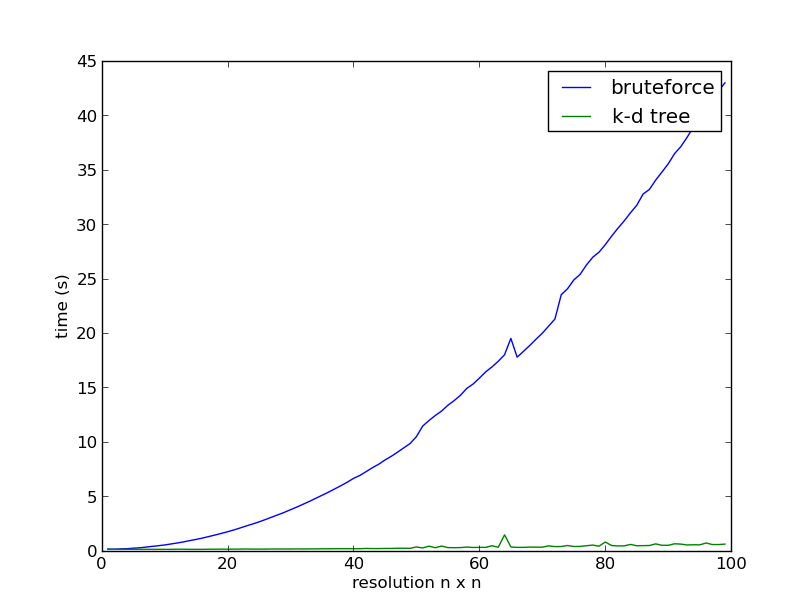
\includegraphics[width=0.7\textwidth]{images/results/tri_intersection.png}
\caption{Comparison of bruteforce and k-d tree mesh intersection test}
\label{fig:bf_kd_comp}
\end{figure}
It can be seen in Figure~\ref{fig:bf_kd_comp} that there are clear gains had from 
using the k-d tree when performing the intersection test, this test was performed
for image resolutions from $1\times1$ to $100\times100$, even for these low
resolution tests we can see how infeasable performing the bruteforce method becomes.
It is clear that implementing the k-d tree acceleration structure is of great
benifit to the system.


\section{Multicore Scaling}
\begin{figure}[h]
\centering
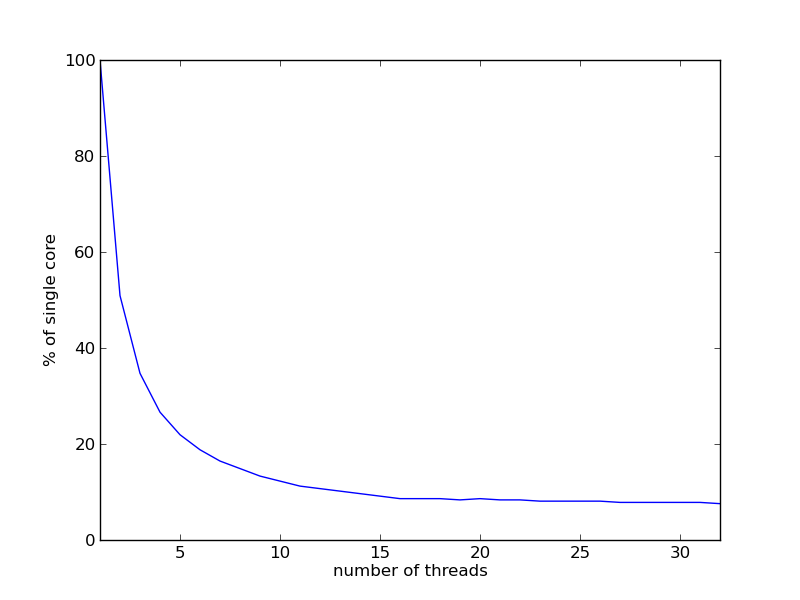
\includegraphics[width=0.7\textwidth]{./images/results/raytrace_multicore.png}
\caption{Raytracing Parrelism Test}
\label{fig:perfraytrace}
\end{figure}

It can be seen from Figure~\ref{fig:perfraytrace} that performance gains were
acheived as cores were added to the system, these results do show that this
part of the system is able to utilise the hardware of even relitivly powerful
machines, we can see that we begin to see diminishing returns on the speedup,
while it would be desirable to improve the system to further utilise the resources
of the machine for the most common use case of a machine with a low number of cores
we see a near linear speedup.

\begin{figure}[h]
\centering
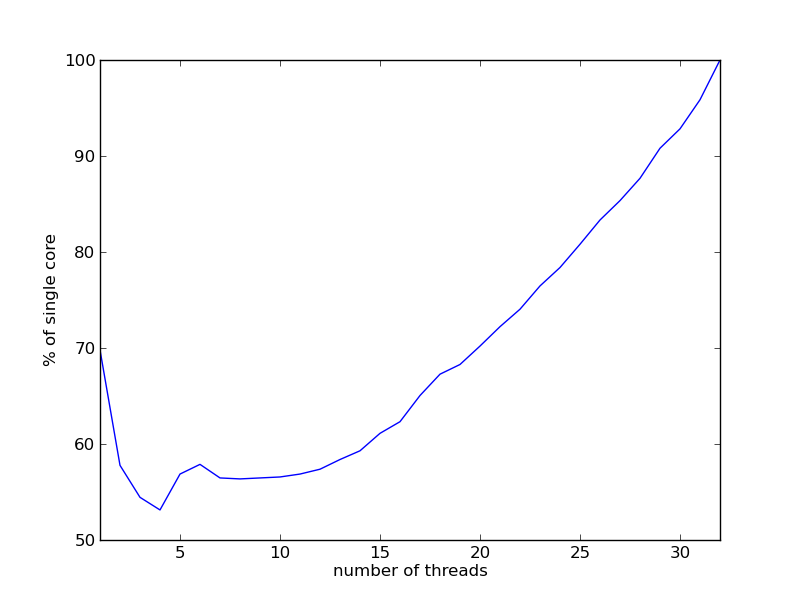
\includegraphics[width=0.7\textwidth]{./images/results/photon_emission_slow_20.png}
\caption{Photon map construction parrelism test}
\label{fig:perfphotonmap}
\end{figure}

The results for the photon map construction test were less impressive, it can be seen
in Figure~\ref{fig:perfphotonmap} that for large
numbers of cores the performance of this part of the system begins to deterierate,
we were not able to in the time frame of the project able to determin the cause of
this behavoir, not least because for core counts of less than five we see that the
system does indeed improve and as the main development machine only has four cores
debugging on this machine was not an option. We beleive that the design of this
componenet of the system was perhaos naive in its approach to parralism and
a more sophisticated desing was needed.

\section{System Output}
In this section we shall present images that were created with the system to
showcase the final product, each rendered scene displays the use of the photon
mapping algorithm and how we have been able to use it to create visually
pleasing images.

\begin{figure}
\centering
	\begin{subfigure}[b]{0.6\textwidth}
		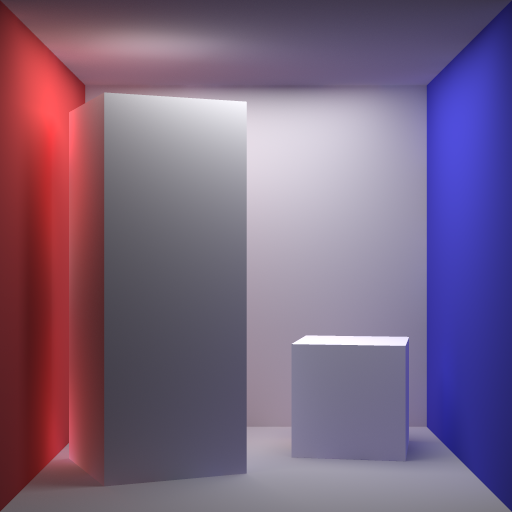
\includegraphics[width=\textwidth]{./images/renders/box.png}
		\caption{Cornell Box (note diffuse reflection of the walls and top of the box on the ceiling)}
	\end{subfigure}
	\begin{subfigure}[b]{0.6\textwidth}
	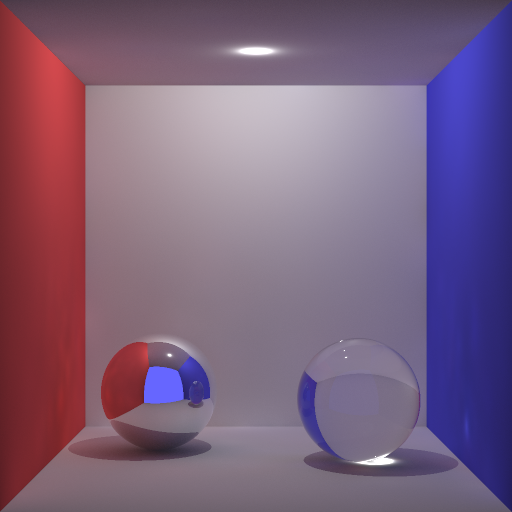
\includegraphics[width=\textwidth]{./images/renders/cornell_box.png}
	\caption{Cornell Spheres (note caustics on the glass sphere)}
	\end{subfigure}
\end{figure}

\begin{figure}
\ContinuedFloat
\centering
	\begin{subfigure}[b]{0.6\textwidth}
	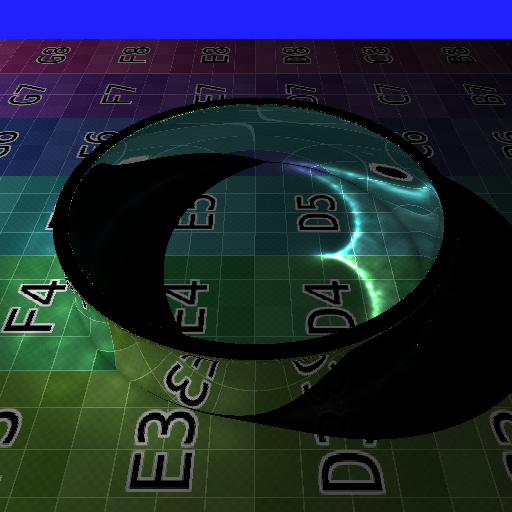
\includegraphics[width=\textwidth]{./images/renders/caustic_ring.png}
	\caption{Caustic Ring}
	\end{subfigure}

	\begin{subfigure}[b]{0.6\textwidth}
	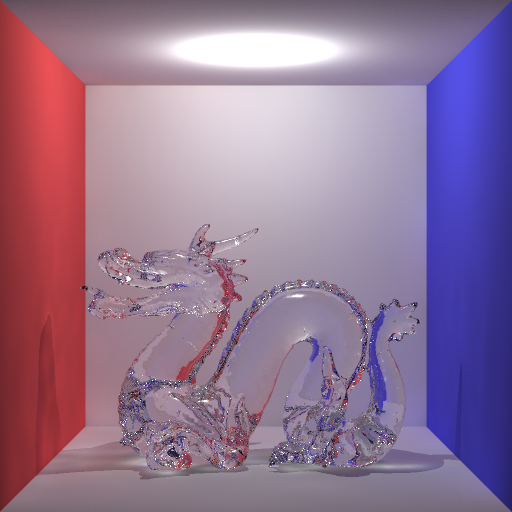
\includegraphics[width=\textwidth]{./images/renders/dragon.png}
	\caption{Stanford Dragon}
	\end{subfigure}
\end{figure}

\begin{figure}
\ContinuedFloat
\centering
	\begin{subfigure}[b]{0.6\textwidth}
	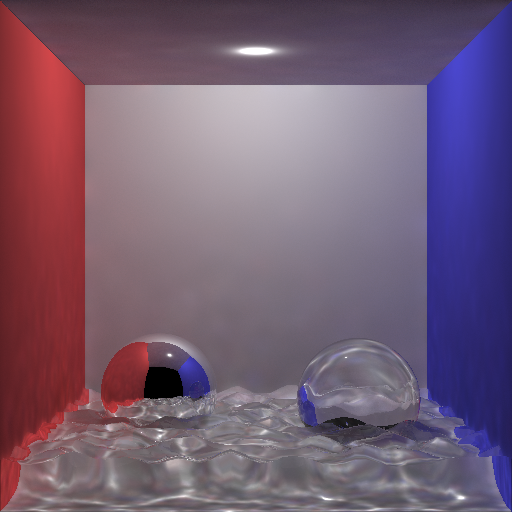
\includegraphics[width=\textwidth]{./images/renders/water.png}
	\caption{Cornell box filled with water (note caustic ripples on the floor)}
	\end{subfigure}

	\begin{subfigure}[b]{0.6\textwidth}
	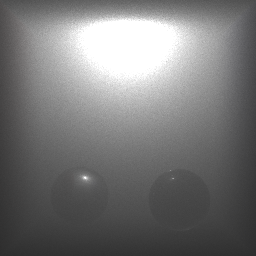
\includegraphics[width=\textwidth]{./images/pmedia.png}
	\caption{Cornell box filled with smoke}
	\end{subfigure}
\end{figure}

